\section{Calentamiento}

Indique lo que imprimen los siguientes programas

\begin{center}
\begin{tabular}{l l}
    \begin{tabularlstlisting}
c = (True and not 7==7.0)
b = False or c
print(b)
    \end{tabularlstlisting}
     & 
    \begin{tabularlstlisting}
c = 13//5
b = 2.5
print(c+b)
    \end{tabularlstlisting}
    \\
    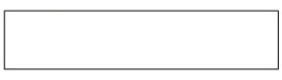
\includegraphics[scale=0.75]{Imagenes/cuadrado} & 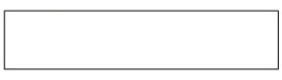
\includegraphics[scale=0.75]{Imagenes/cuadrado} \\
    \begin{tabularlstlisting}
n = 'Sed ut perspiciatis unde'
b = n.replace('i', 'o', 2)
print(b.split()[2][3:9])
    \end{tabularlstlisting}
     & 
    \begin{tabularlstlisting}
refran = 'Al mal tiempo, buena cara.'
c = refran.split()[::3]
print('\n'.join(c))
    \end{tabularlstlisting}
    \\
    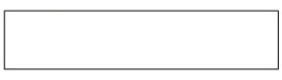
\includegraphics[scale=0.75]{Imagenes/cuadrado} & 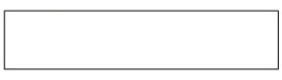
\includegraphics[scale=0.75]{Imagenes/cuadrado} \\
    \begin{tabularlstlisting}
n = 483
while n / 10.0 != 0:
    d = n % 10
    n /= 10
print(d)
    \end{tabularlstlisting}
     & 
    \begin{tabularlstlisting}
def f3(a):
    return a[1]

a = [0, 1, 2]
b = {0:1, 1:2}
print(f3(b))
    \end{tabularlstlisting}
    \\
    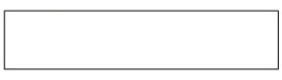
\includegraphics[scale=0.75]{Imagenes/cuadrado} & 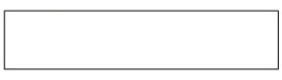
\includegraphics[scale=0.75]{Imagenes/cuadrado} \\
\end{tabular}
\end{center}

